%% Audio-Visual Cross-Attention and Facial-Behavior Fusion for Ordinal Student Engagement Recognition — IEEE journal draft
%% Based on bare_jrnl.tex V1.4b (Michael Shell, IEEEtran).
%% Section order: Introduction / Related Work / Preliminaries / Proposed Research Method /
%% Experimental Details / Model Evaluation / Conclusion.

\documentclass[journal]{IEEEtran}

\usepackage{cite}
\usepackage{graphicx} % driver auto-detected (pdfLaTeX, XeLaTeX, LuaLaTeX)
\graphicspath{{figures/}}
\usepackage{amsmath}
\usepackage{amssymb}
\usepackage{algorithmic}
\usepackage{algorithm}
\usepackage{tikz}
\usetikzlibrary{positioning,calc,decorations.pathreplacing}
\usepackage{pgfplots}
\pgfplotsset{compat=1.17}
% Shared figure colours (validated for colour-vision deficiency; see dataviz palette).
\definecolor{ours}{HTML}{2A78D6}      % our single models
\definecolor{fused}{HTML}{EB6834}     % our late fusion
\definecolor{published}{HTML}{8F8E88} % published EngageNet baselines
\definecolor{inkmuted}{HTML}{52514E}
\definecolor{boxfill}{HTML}{F3F2EF}
\definecolor{seqlo}{HTML}{FFFFFF}
\definecolor{seqhi}{HTML}{104281}


\hyphenation{op-tical net-works semi-conduc-tor}

\begin{document}

\title{Audio-Visual Cross-Attention and Facial-Behavior Fusion for Ordinal Student Engagement Recognition}

\author{Name%
% Add final affiliation, email addresses, and manuscript dates here if required
% by the target IEEE venue.
}

\markboth{IEEE Journal Draft}%
{Gupta and Ghose: Audio-Visual and Facial-Behavior Fusion for Ordinal Engagement Recognition}

\maketitle

\begin{abstract}
Automatic student engagement recognition can help instructors see when students are attentive, partially engaged, or disengaged during online learning, but engagement is expressed through several behaviors at once and is annotated on an ordered scale. Published results on EngageNet, the public online-learning engagement corpus with the most participants, use video only, report top-1 accuracy, and do not state how class probabilities are turned into a level. We present an audio-visual engagement recogniser that pools the audio token sequence onto the visual frame grid of each clip before two-stage cross-attention, trains with an ordinal distance penalty, and decodes the expected engagement level with thresholds fitted on the validation split. On the EngageNet test split the audio-visual network reaches 66.27 $\pm$ 0.45\% top-1 accuracy over three seeds; audio alone carries no clip-level signal, yet removing it from the trained model lowers accuracy in eight of nine matched runs (mean 0.74 points). Calibrated decoding adds 2.0 points on identical weights. An explicit OpenFace behavior branch inside the network changes no metric, whereas two shallow models on segment statistics of the same OpenFace features make errors that differ from the network's: averaging the three probability distributions with fixed weights reaches 70.29 $\pm$ 0.14\% top-1, 91.1\% adjacent accuracy and a mean absolute class error of 0.40, 2.7 points above the best published test-split EngageNet result. We report adjacent accuracy, mean absolute class error and macro-F1 alongside top-1 together with a seed noise floor, and show that most remaining errors lie between the two middle engagement levels.
\end{abstract}

\begin{IEEEkeywords}
Student engagement, multimodal learning, online education, audio-visual fusion, ordinal classification.
\end{IEEEkeywords}

\IEEEpeerreviewmaketitle


\section{Introduction}

\IEEEPARstart{S}{tudent} engagement is a key indicator of learning quality in online and hybrid classrooms. An engaged student is not only present in a session, but is also attentive, responsive, and involved in the learning activity. In face-to-face teaching, instructors judge this state by observing several forms of behavior together, including facial expression, posture, eye contact, speech, and interaction with classmates. In online learning, these signals become harder to interpret because students appear through webcams, microphones may be muted, and the instructor has limited access to the full classroom environment. For this reason, automatic student engagement recognition has become an important problem in educational technology and affective computing \cite{qarbal2025review}.

The main difficulty is that engagement is not expressed through one modality or one fixed behavior. Many engagement-recognition methods rely heavily on visual information such as face images, head pose, gaze direction, and facial action units. These features can capture visible attention, but they may not fully represent a student's learning state. A student may look at the screen without actively following the lesson, while another student may look away briefly while thinking. Audio can provide additional evidence through speaking activity, hesitation, tone, and participation patterns. However, existing online engagement datasets often contain limited or uneven speech, which makes audio difficult to use consistently. As a result, the boundary between disengaged and engaged states remains challenging, especially when both attentive listening and passive disengagement appear visually quiet \cite{singh2023engagenet,wu2024cmose}. Fig.~\ref{fig_concept} summarises the problem on EngageNet: three sources of evidence must be combined into one ordered level, and the two middle levels, which describe a difference of degree in similar visible behavior, account for most of the errors.

\begin{figure}[!t]
\centering
\resizebox{\columnwidth}{!}{% Fig. 1 — problem framing (Introduction). Shares are the EngageNet test split (n = 2,256);
% the error share is the audio-visual network pooled over its three seeds.
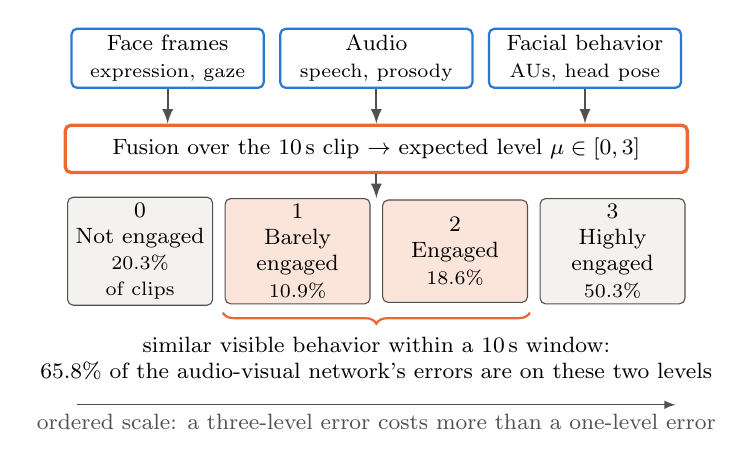
\begin{tikzpicture}[font=\footnotesize, >=latex,
  lvl/.style={draw=inkmuted, fill=boxfill, rounded corners=2pt, text width=1.7cm, minimum height=1.3cm, align=center, inner sep=2pt},
  cue/.style={draw=ours, thick, rounded corners=2pt, text width=2.3cm, minimum height=0.75cm, align=center, fill=white, inner sep=2pt}]
  \node[cue] (v) at (0.35,2.45) {Face frames\\\scriptsize expression, gaze};
  \node[cue] (a) at (3.0,2.45) {Audio\\\scriptsize speech, prosody};
  \node[cue] (b) at (5.65,2.45) {Facial behavior\\\scriptsize AUs, head pose};
  \node[draw=fused, very thick, rounded corners=2pt, minimum width=7.9cm, minimum height=0.6cm, fill=white] (m) at (3.0,1.3)
     {Fusion over the 10\,s clip $\rightarrow$ expected level $\mu\in[0,3]$};
  \foreach \s in {v,a,b} \draw[->, thick, inkmuted] (\s) -- (\s |- m.north);
  \node[lvl] (l0) at (0,0)   {0\\Not engaged\\\scriptsize 20.3\% of clips};
  \node[lvl, fill=fused!18] (l1) at (2.0,0) {1\\Barely engaged\\\scriptsize 10.9\%};
  \node[lvl, fill=fused!18] (l2) at (4.0,0) {2\\Engaged\\\scriptsize 18.6\%};
  \node[lvl] (l3) at (6.0,0) {3\\Highly engaged\\\scriptsize 50.3\%};
  \draw[->, thick, inkmuted] (m.south) -- (m.south |- l1.north);
  \draw[decorate, decoration={brace, amplitude=4pt, mirror}, fused, thick] (1.05,-0.78) -- (4.95,-0.78)
     node[midway, below=5pt, text=black, align=center]{similar visible behavior within a 10\,s window:\\ 65.8\% of the audio-visual network's errors are on these two levels};
  \draw[->, inkmuted] (-0.8,-1.95) -- node[below, text=inkmuted]{ordered scale: a three-level error costs more than a one-level error} (6.8,-1.95);
\end{tikzpicture}
}
\caption{Problem framing. Face, audio and facial-behavior evidence from a 10\,s clip is fused into an expected level on the ordered four-level EngageNet scale. Percentages are the share of each level in the test split (2,256 clips). The two middle levels are both rare and visually similar; they receive 65.8\% of the errors of our audio-visual network (three seeds pooled).}
\label{fig_concept}
\end{figure}

To address this problem, this paper develops a multimodal audio-video framework for online student engagement recognition. The visual branch extracts facial and temporal behavior from video frames, while the audio branch extracts speech-related information from the corresponding audio signal. The two streams are combined through an audio-video attention mechanism inspired by cross-attention methods used in multimodal emotion recognition \cite{venkatraman2025avtca}. This design allows the model to learn complementary information from both modalities instead of depending only on a single visual stream. Because a network trained end to end on 7,879 clips does not extract everything that explicit facial-behavior descriptors contain, we combine it at the probability level with two shallow models built on segment statistics of OpenFace action-unit, gaze and head-pose features. The framework also treats engagement as an ordered learning state because datasets commonly describe engagement using levels such as highly disengaged, disengaged, engaged, and highly engaged \cite{wu2024cmose,tran2026ordinal}.

The experiments test whether audio-video fusion improves engagement recognition over the video-only condition of the same trained model, and whether explicit behavior features add information that the network does not already use. In addition to standard classification metrics, the evaluation includes ordered-label measures such as adjacent accuracy and mean absolute class error. These metrics are important because they show not only whether the model predicts the exact class, but also how far the prediction is from the true engagement level. This is especially useful for analyzing errors between nearby classes, where the distinction is often subtle.

This paper claims that online student engagement recognition should be modeled as a multimodal and ordered-state prediction problem, closer to how instructors judge students in real classrooms: by considering several behaviors together over time rather than a single visible signal. The main contributions of this work are summarized as follows:
\begin{itemize}
\item We present, to our knowledge, the first audio-visual model evaluated on EngageNet, where all published baselines are video-only. Audio alone is no better than the majority-class predictor on this corpus, yet removing the audio stream from the trained model lowers top-1 accuracy in eight of nine matched runs (mean $-0.74$ points), so audio contributes through cross-modal interaction rather than as an independent predictor.
\item We pool the audio token sequence of each clip adaptively onto the visual frame grid of the same clip before the first cross-attention block, so that the two modalities exchange information at the same temporal resolution for clips of any length.
\item We decode the four engagement levels with calibrated ordinal thresholds on the expected level, fitted on the validation split. On identical weights this adds 2.0 points of top-1 accuracy over argmax (three seeds), which shows that the decoding rule must be stated for engagement accuracies to be comparable across papers.
\item We show that an explicit OpenFace behavior branch inside the network changes no metric over three seeds, whereas shallow models on segment statistics of the same 22 features make errors that differ from the network's. Fixed-weight probability averaging of the network with two such models reaches 70.29 $\pm$ 0.14\% top-1, 2.7 points above the best published test-split EngageNet result.
\item We report adjacent accuracy, mean absolute class error and macro-F1 next to top-1 accuracy, together with a three-seed noise floor, and show with a matched single-variable sweep that the remaining error is concentrated between the two middle engagement levels.
\end{itemize}
The remainder of this paper is organized as follows. Section~\ref{sec:relwork} reviews related work. Section~\ref{sec:prelim} defines the attention operation, the ordinal label formulation, and the evaluation measures. Section~\ref{sec:method} describes the proposed architecture, Section~\ref{sec:exp} the datasets and training protocol, and Section~\ref{sec:eval} the quantitative results, ablation analysis, error analysis, and human evaluation.

\section{Related Work}
\label{sec:relwork}

\subsection{Student Engagement Recognition}

Student engagement recognition has been studied using computer vision, machine learning, and multimodal learning methods. Traditional engagement assessment often depends on instructor observation, self-report surveys, or manual coding. Although these methods can provide useful information, they are difficult to scale and may be subjective. For this reason, recent research has focused on automatic engagement detection using video, audio, behavior logs, and classroom interaction data \cite{qarbal2025review,theophilus2026review}. A recent review of 48 studies compares shallow and deep learning approaches to learner engagement prediction and organises them by how features are selected, extracted and engineered \cite{theophilus2026review}. On DAiSEE, gradient boosting on OpenFace action units has been reported to outperform an end-to-end convolutional network by a wide margin \cite{das2025optimizing}, an early indication that explicit facial-behavior features remain competitive with learned frame encoders on engagement corpora of this size.

Many early systems used visual features because face and body behavior are easy to capture from classroom or webcam videos. Common visual cues include facial expression, eye gaze, head pose, posture, and facial action units. These features can provide strong signals of attention and participation. However, vision-only systems also have limitations. They can be affected by lighting, camera angle, occlusion, and individual differences in expression. More importantly, visible attention is not always the same as cognitive engagement. A student may appear focused but not be mentally involved, while another student may look away briefly while thinking.

DAiSEE is one of the commonly used datasets for engagement recognition in online learning. It provides video clips labeled with engagement-related states and has been used to test several baseline models \cite{gupta2016daisee}. However, DAiSEE also shows common challenges in this area, including class imbalance, short clip-based labeling, and difficulty in judging internal student states from video alone. These issues make it difficult for models trained on one dataset to generalize well to real classroom settings. Class imbalance in particular has motivated dedicated remedies: generative augmentation of the under-represented low-engagement classes on EngageNet improves macro-F1 without a loss in overall accuracy \cite{yulius2025gan}, which indicates that minority-level performance is a distinct problem from headline accuracy.

EngageNet extends this direction by providing a larger engagement dataset collected in more diverse conditions \cite{singh2023engagenet}. It includes participants under different illumination and recording settings and evaluates features such as action units, gaze, head pose, and learned visual representations. The results show that engagement prediction remains challenging even with larger datasets, especially when the model must handle real-world variation. This supports the need for robust multimodal models rather than relying only on one type of visual cue. The EngageNet authors also note that noise and missing audio led them to concentrate on video only \cite{singh2023engagenet}. Along the same line, MSC-Trans fuses several visual feature groups through a transformer encoding structure and shows that fixed feature combinations limit classroom engagement detection \cite{xie2025msctrans}, and GLP-fusion proposes a hierarchical multimodal fusion framework for robust engagement prediction \cite{qin2026glpfusion}.

Work published after EngageNet has continued on the same corpus, almost always with visual or facial-behavior input and with results reported on the validation split, because the test labels were not publicly released. TCCT-Net estimates engagement from OpenFace head-pose signals with a two-stream convolution-transformer network and reports 68.91\% validation accuracy \cite{vedernikov2024tcct}; an ordinal spatial-temporal graph network on facial landmarks reaches 71.24\% \cite{abedi2024stgcn}; PriorNet, a prior-guided face-video model, reports 73.58\% \cite{vedernikov2026priornet}; and a variational encoder with multiple decoders, which has an audio branch for other corpora, is evaluated on EngageNet with video only (68.98\%) \cite{augusma2026vemd}. Vision-language models have also been used to refine noisy EngageNet labels, improving several feature settings by up to 1.2 points \cite{vedernikov2025vlmnoise}, which is consistent with annotation noise being a limit on this corpus. On DAiSEE, a face-and-scene spatio-temporal network reports 73.43\% test accuracy \cite{gothwal2025vibednet}. None of these studies uses the audio track of EngageNet.

CMOSE further highlights the importance of label quality and multimodal information for online student engagement recognition \cite{wu2024cmose}. It addresses problems such as poor label quality, class imbalance, and large variation within the same engagement class. CMOSE also shows that speech and audio features can improve engagement prediction when they are available. This is important for online collaborative learning because participation is not only visual; it is also expressed through speaking behavior, hesitation, tone, and interaction. A recent framework that integrates visual, audio, physiological and behavior-log streams with a bidirectional LSTM reports that multimodal fusion outperforms vision-only and late-fusion baselines on CMOSE by a clear macro-F1 margin \cite{zhao2026multimodal}, again pointing to the under-represented levels as the place where additional modalities pay off.

\subsection{Multimodal Audio-Visual Learning}

Multimodal learning is useful because human behavior is naturally expressed through more than one channel. In affective computing and emotion recognition, audio provides information about tone, intensity, rhythm, and hesitation, while video provides information about facial expression, movement, and visual attention. Combining these modalities can make the model more reliable than using only one source. Surveys of multimodal emotion recognition organise the field by fusion level and by how a model behaves when one modality is missing or weak \cite{li2026mersurvey}, which is precisely the situation in online classrooms where microphones are frequently muted. Deep convolutional and recurrent fusion of face and speech remains a strong and widely used baseline for audio-visual emotion recognition \cite{taware2025mer}, and related multimodal architectures combine text and audio for sentiment polarity detection \cite{hegde2025sentiment} and to depression recognition from audio, video and text \cite{lu2026dstc}, where the DSTC network explicitly models modality differences before fusion.

Audio-video fusion has been widely studied in multimodal emotion recognition. AVT-CA uses transformer-based cross-attention to combine audio and visual information \cite{venkatraman2025avtca}. In this type of model, audio features can attend to visual features, and visual features can attend to audio features. This is useful because it allows the model to learn which parts of one modality support or correct the other modality. For student engagement recognition, this idea is helpful because audio and video may not always be equally reliable. For example, video may be unclear due to lighting or face occlusion, while audio may be missing or weak when students are silent.

Recent audio-visual fusion work also shows that the level of fusion matters. Some methods use late fusion, where separate audio and visual predictions are combined near the end. Other methods use early fusion, where audio and visual tokens interact earlier in the model. Early fusion can capture fine-grained relationships, but it may require more data and computation \cite{mo2024earlyfusion}. Attention bottleneck methods try to reduce unnecessary cross-modal interaction while still keeping the most useful information \cite{nagrani2021attention}. Transformer fusion of audio and visual streams has also been shown to improve action recognition over either modality alone when the streams are first converted to a common representation format and fused with co-attention \cite{kim2024avaction}; our alignment module addresses the related requirement that the two token sequences cover the same time span at the same resolution. These studies suggest that a practical engagement-recognition system should use multimodal fusion carefully instead of adding complexity without a clear reason.

\subsection{Ordinal and Context-Aware Engagement Modeling}

Engagement labels are usually ordered. For example, a four-level engagement scale may include highly disengaged, disengaged, engaged, and highly engaged. Treating these labels as unrelated classes ignores the natural order between them. A prediction error between engaged and highly engaged should not be treated the same as an error between highly disengaged and highly engaged. Therefore, ordinal modeling is important for engagement recognition.

Recent work has started to address this issue. CMOSE proposes a training strategy that considers the ordinal pattern of engagement levels \cite{wu2024cmose}. CORE-Net also uses ordinal supervision and context modeling for collaborative learning \cite{tran2026ordinal}. Ordinal formulations over affect and OpenFace behavior features improve engagement measurement on DAiSEE \cite{abedi2024affect,safa2025sclordinal}, and on EngageNet an ordinal graph network improves on its non-ordinal counterpart \cite{abedi2024stgcn}. These methods build the ordering into training; our work adds it at decoding time as well and quantifies what the decoding rule alone contributes. These studies show that engagement should not be modeled only as a standard classification problem. Instead, the model should understand both the order of labels and the classroom context in which behavior occurs.

Context is especially important in collaborative learning. Student engagement does not depend only on one student's face or voice. It is also influenced by the learning activity, group interaction, and the student's role in the conversation. A behavior that appears disengaged in one context may be normal or even productive in another context. For example, silence can indicate disengagement when a student is expected to speak, but it can also indicate active listening when another student is speaking.

Some recent models use richer context and hierarchical fusion to improve engagement prediction. GLP-fusion uses a hierarchical multimodal fusion strategy \cite{qin2026glpfusion}. CORE-Net models group-level context for collaborative learning \cite{tran2026ordinal}. These methods show that engagement recognition benefits from information beyond a single facial frame. However, most existing models still do not directly treat speaker-listener role as a central part of the prediction process.

\subsection{Research Gap}

The reviewed studies show important progress in student engagement recognition, but several gaps remain. First, many models still depend mainly on visual information, even though audio and speech behavior can provide useful evidence of participation and confusion. Second, engagement is often treated as a flat class label, even though engagement levels are ordered. Third, current systems rarely model the student's conversational role. In collaborative learning, the same gaze, silence, or speech pattern can have different meanings depending on whether the student is speaking or listening.

This paper addresses the first two gaps directly: it fuses audio with video and with explicit facial-behavior features, and it trains and decodes engagement as an ordered level. The third gap, the student's conversational role, cannot be tested on EngageNet, whose clips carry no speaker or listener annotation. We therefore do not claim role conditioning here; the error analysis in Section~\ref{sec:eval} shows why it is the natural next step, and the human evaluation protocol is designed to collect the speaking-or-listening information that the current corpus lacks.

\section{Preliminaries}
\label{sec:prelim}

This section defines the notation used in the rest of the paper. It
describes the attention operation that joins the two modalities, the
ordered form of the engagement labels, and the measures used to evaluate
the predictions.

\subsection{Multi-Head Cross-Attention}
\label{sec:prelim_mha}

Let the audio stream be $X_a \in \mathbb{R}^{T_a \times d_a}$ and the
video stream be $X_v \in \mathbb{R}^{T_v \times d_v}$, where $T_a$ and
$T_v$ are the number of time steps produced by each encoder and $d_a$ and
$d_v$ are their feature sizes. The two streams do not have to share a
feature size, because the projections below map them into a common output
size $d_o$.

Scaled dot-product attention maps a query matrix $Q$, a key matrix $K$,
and a value matrix $V$ to

\begin{equation}
\mathrm{Att}(Q,K,V) = \mathrm{softmax}\!\left(\frac{QK^{\top}}
{\sqrt{d_h}}\right) V
\end{equation}

where $d_h = d_o / h$ is the size of one attention head. Multi-head
attention applies this operation $h$ times in parallel with separate
learned projections and concatenates the results,

\begin{equation}
\mathrm{head}_i = \mathrm{Att}\!\left(X_q W_i^{Q},\; X_k W_i^{K},\;
X_k W_i^{V}\right)
\end{equation}
\begin{equation}
\mathrm{MHA}(X_q, X_k) = \left[\mathrm{head}_1, \ldots,
\mathrm{head}_h\right] W^{O}
\end{equation}

where $X_q$ is the stream that supplies the queries and $X_k$ the stream
that supplies the keys and the values. The projection matrices are
$W_i^{Q} \in \mathbb{R}^{d_q \times d_h}$, $W_i^{K}, W_i^{V} \in
\mathbb{R}^{d_k \times d_h}$, and $W^{O} \in \mathbb{R}^{d_o \times
d_o}$, so the query and key streams may enter with different feature
sizes.

In self-attention the queries and the keys come from the same stream. In
cross-attention they come from different streams. The two cross-modal
directions are

\begin{align}
\tilde{X}_a &= X_a + \mathrm{MHA}(X_a, X_v) \label{eq:xattn_a}\\
\tilde{X}_v &= X_v + \mathrm{MHA}(X_v, X_a) \label{eq:xattn_v}
\end{align}

The residual term keeps the original stream available when the other
modality is uninformative. Each attention block used in Section~\ref{sec:method} also
applies layer normalisation to its inputs and a feed-forward sublayer to
its output; these are omitted from (\ref{eq:xattn_a}) and (\ref{eq:xattn_v}) for readability.

The attention matrix inside (\ref{eq:xattn_a}) has shape $T_a \times T_v$. Every audio
step is compared against every video step, so the two lengths do not have
to match for the operation to be defined. They do, however, have to
describe the same span of time at a comparable resolution. Section~\ref{sec:method}
returns to this point.

\subsection{Ordinal Engagement Labels}
\label{sec:prelim_ordinal}

Engagement is annotated on an ordered scale. We write the label set as
$\mathcal{L} = \{0, 1, \ldots, K-1\}$ with $K = 4$, where larger values
mean higher engagement. For a clip with label $y \in \mathcal{L}$, the
model produces a vector of logits $z \in \mathbb{R}^{K}$, converted to
class probabilities by the softmax function,

\begin{equation}
p_k = \frac{\exp(z_k)}{\sum_{j} \exp(z_j)}
\end{equation}

The usual decision rule takes the largest probability,

\begin{equation}
\hat{y} = \arg\max_{k} \; p_k \label{eq:argmax}
\end{equation}

This rule treats the four levels as unrelated categories. It uses the
value of each probability but not the position of the class on the scale,
so predicting level 0 for a true level 3 is treated the same as
predicting level 2.

An ordered alternative first reduces the probability vector to a single
number on the engagement scale, which we call the expected level,

\begin{equation}
\mu = \sum_{k=0}^{K-1} k \, p_k \label{eq:mu}
\end{equation}

and then cuts it with a set of increasing thresholds
$\tau_1 < \tau_2 < \cdots < \tau_{K-1}$,

\begin{equation}
\hat{y} = \sum_{m=1}^{K-1} \mathbf{1}\!\left[\mu \geq \tau_m\right] \label{eq:thresh}
\end{equation}

where $\mathbf{1}[\cdot]$ is the indicator function. The thresholds are
fitted on the validation split and are not learned during training.
Equations (\ref{eq:argmax}) and (\ref{eq:thresh}) agree when the probability vector is sharply peaked
and the thresholds separate consecutive levels, and can differ when the
probability mass is spread across neighbouring levels.

The ordering can also be used during training. We add to the
cross-entropy loss a penalty that grows with the distance between the
predicted and the true level,

\begin{equation}
\mathcal{L} = \mathcal{L}_{\mathrm{CE}} + \lambda \sum_{k} p_k
\left| c_k - c_y \right|, \qquad c_k = \frac{k}{K-1} \label{eq:loss}
\end{equation}

where $\mathcal{L}_{\mathrm{CE}}$ is cross-entropy with label smoothing.
Class positions are normalised to $[0,1]$ so that $\lambda$ has the same
meaning for any $K$. The weight $\lambda$ controls how strongly the
distance term counts against the cross-entropy term.

\subsection{Evaluation Measures}
\label{sec:prelim_metrics}

Let $N$ be the number of test clips, with true labels $y_i$ and
predictions $\hat{y}_i$. We report four measures. Top-1 accuracy is the
fraction of clips whose level is predicted exactly, adjacent accuracy is
the fraction predicted within one level, and mean absolute class error
(MAE) is the average distance in levels,

\begin{align}
\mathrm{Top\text{-}1} &= \frac{1}{N} \sum_{i=1}^{N}
\mathbf{1}\!\left[\hat{y}_i = y_i\right] \\
\mathrm{Adj} &= \frac{1}{N} \sum_{i=1}^{N}
\mathbf{1}\!\left[\left|\hat{y}_i - y_i\right| \leq 1\right] \\
\mathrm{MAE} &= \frac{1}{N} \sum_{i=1}^{N}
\left|\hat{y}_i - y_i\right|
\end{align}

Macro-F1 is the F1 score computed for each level and then averaged over
levels with equal weight. It is reported because the levels are
unbalanced: a model that always predicts the most common level reaches
50.27\% top-1 accuracy on this dataset but only 16.73 macro-F1.

Top-1 accuracy is the standard measure in the engagement literature. It
gives no credit for a near miss, and it charges the same amount for an
error of one level as for an error of three. Adjacent accuracy and MAE
record the size of the error, and are therefore reported next to top-1
throughout this paper.

\section{Proposed Research Method}
\label{sec:method}

We separate the proposed system into five components: A) an audio encoder, B) a visual encoder, C) a temporal alignment and two-stage cross-attention fusion module, D) an ordinal prediction head with calibrated decoding, which together form the audio-visual network, and E) two facial-behavior statistics models that are combined with the network at the probability level. We explain each component in the following subsections. The complete pipeline is shown in Fig.~\ref{fig_arch}.

% Source: figures/architecture.drawio (edit in draw.io, export PDF with "crop" to figures/architecture.pdf).
\begin{figure*}[!t]
\centering
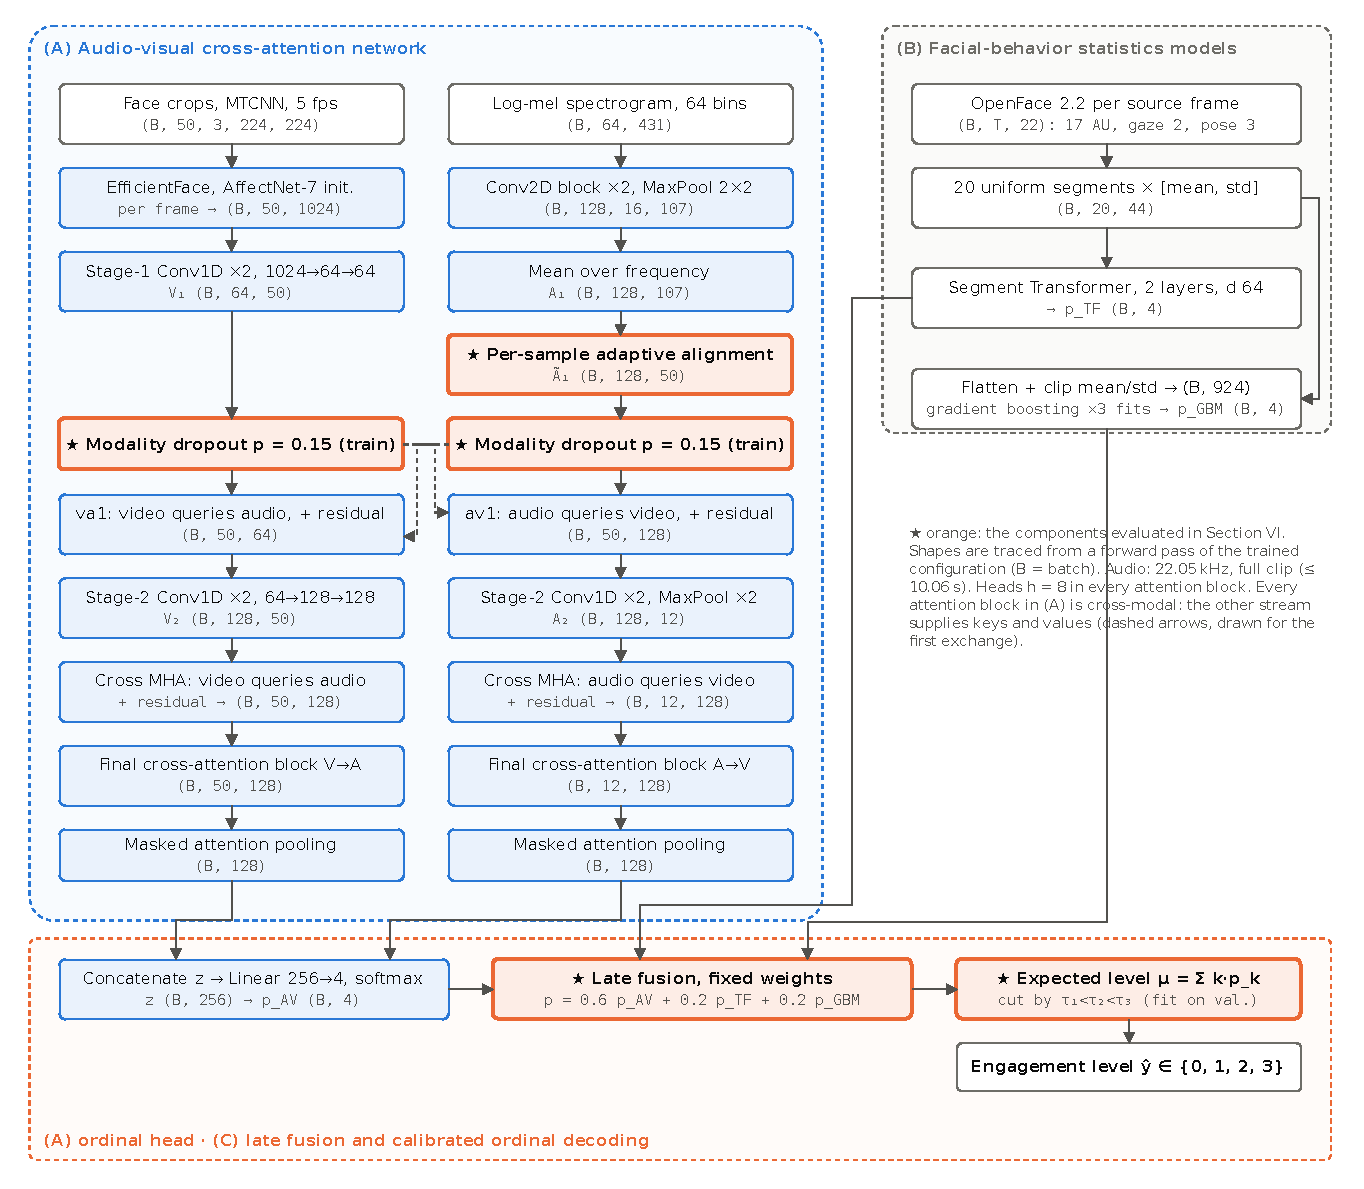
\includegraphics[width=\textwidth]{architecture}
\caption{Overview of the proposed engagement recogniser; tensor shapes are traced from a forward pass ($B$ = batch). (A)--(C) The audio-visual network: audio tokens are pooled onto the 50-step visual clock of the same clip before the first cross-attention exchange; after the second convolutional stage the audio stream is downsampled to 12 tokens while the video stream keeps 50; every attention block is cross-modal. (E, top right) Two models on segment statistics of the per-frame OpenFace descriptor. (D, E, bottom) The three class-probability vectors are averaged with fixed weights, collapsed to an expected level, and cut by thresholds fitted on the validation split. Orange blocks mark the components evaluated in Section~\ref{sec:eval}.}
\label{fig_arch}
\end{figure*}

\subsection{Audio Encoder}

The audio branch receives the full 10\,s waveform of each clip, resampled to 22.05\,kHz and converted to a 64-bin log-mel spectrogram $\mathbf{X}_a \in \mathbb{R}^{64 \times T_a}$. A two-dimensional convolutional stack operates jointly over the frequency and time axes, after which the frequency axis is collapsed by averaging, producing a sequence of 128-dimensional temporal tokens at one quarter of the input frame rate. This sequence is the first-stage audio representation $\mathbf{A}_1 \in \mathbb{R}^{128 \times T_a/4}$. A second stage of two one-dimensional convolutions (128$\to$256$\to$128 channels) is applied after the first cross-attention exchange and yields $\mathbf{A}_2$. Mel-spectrogram input was preferred to MFCC features because the convolutional front end can learn its own frequency pooling, and because the 64-bin representation preserves the prosodic contours (pitch movement, energy envelope) that carry speaking activity and hesitation information.

\subsection{Visual Encoder}

\subsubsection{Visual Frame Encoder}
Each clip is sampled at 5 frames per second, giving up to 50 face crops of $224 \times 224$ pixels detected with MTCNN. Every frame is encoded independently by an EfficientFace backbone \cite{zhao2021efficientface} composed of inverted-residual blocks with a channel-and-spatial modulator, initialised from weights pre-trained on AffectNet-7. The backbone maps each frame to a 1024-dimensional embedding. The per-frame embeddings are stacked along time and passed through two one-dimensional convolutions (1024$\to$64$\to$64) that model short-range temporal dynamics, producing the first-stage visual token sequence $\mathbf{V}_1 \in \mathbb{R}^{64 \times T_v}$ with $T_v \le 50$. A second convolutional stage (64$\to$128$\to$128) produces $\mathbf{V}_2$.

\subsubsection{Neural Behavior Branch (Ablation)}
We also evaluated an explicit behavior branch inside the network. OpenFace \cite{baltrusaitis2018openface} is run on the source video of each clip and gives, per frame, 17 facial action unit intensities, two gaze angles, and three head-pose rotations, resampled onto the 50-step visual clock to give a 22-channel sequence $\mathbf{B} \in \mathbb{R}^{22 \times T_v}$. The sequence is encoded by a one-dimensional convolution (22$\to$128) and a bidirectional GRU; the audio-visual summary $\mathbf{z}$ is projected to a query that attends over these tokens, and the clip-mean of the raw descriptor is passed through a linear layer with ReLU to a 64-dimensional skip vector. The classifier then acts on the concatenation of $\mathbf{z}$, the behavior context vector, and the skip vector, and a learned missing-modality token replaces the context vector when no face is found. Section~\ref{sec:ablation} shows that this branch leaves every metric unchanged; the behavior features are therefore used through component E instead, and the branch is not part of the reported system.

% Akshit's visual-emphasis variant — commented out until a matched number exists (plan.md §18.4).
%\subsubsection{Visual-Weighted Fusion Variant}
%Because most EngageNet clips contain no speech, we also evaluate a variant in which the visual summary receives a larger weight at the fusion point. This variant is corpus-specific; the equal-contribution design is retained for speech-rich classroom data.

\subsection{Temporal Alignment and Two-Stage Cross-Attention Fusion}

\subsubsection{Per-Sample Temporal Alignment}
After the first convolutional stage the audio sequence contains 107 time steps for a 10\,s clip whereas the visual sequence contains at most 50. If cross-attention is applied directly, each visual token must attend over about two audio tokens that describe the same instant, and the attention weights spread over a smeared view of the other modality; for the shorter audio windows used in earlier emotion-recognition work the ratio exceeds ten to one. We therefore pool the valid audio span of every sample adaptively onto the valid visual length of the same sample,
\begin{equation}
\tilde{\mathbf{A}}_1[:, j] = \frac{1}{|S_j|}\sum_{t \in S_j} \mathbf{A}_1[:, t], \qquad j = 1,\dots,T_v^{(i)},
\end{equation}
where $S_j$ is the $j$-th of $T_v^{(i)}$ equal-width windows over the valid audio steps of sample $i$. Padding frames are excluded from both sides before pooling and re-masked afterwards, so the alignment is exact for clips of any length. Both streams then meet at the same temporal granularity before the first attention exchange.

\subsubsection{Two-Stage Cross-Attention}
Fusion follows the intermediate-token scheme of AVT-CA \cite{venkatraman2025avtca} with the multi-head attention of Section~\ref{sec:prelim_mha} throughout ($h = 8$ heads). In the first stage the aligned audio tokens query the visual tokens and the visual tokens query the audio tokens, exactly as in (\ref{eq:xattn_a}) and (\ref{eq:xattn_v}) with $X_a = \tilde{\mathbf{A}}_1$ and $X_v = \mathbf{V}_1$; the residual connection preserves each modality's own evidence. Each stream then passes through its second convolutional stage, which brings the audio tokens to $\mathbf{A}_2 \in \mathbb{R}^{128 \times 12}$ and the visual tokens to $\mathbf{V}_2 \in \mathbb{R}^{128 \times 50}$. In the second stage the two streams exchange information twice more: a multi-head cross-attention layer in each direction with residual dropout, followed by a final pair of cross-attention blocks. Each stream is reduced over time to a 128-dimensional vector by learned attention pooling, in which a linear scoring layer produces one weight per valid time step and the tokens are averaged under those weights. Padded steps are masked out of the pooling. The two vectors are concatenated into the 256-dimensional audio-visual summary $\mathbf{z}$. The per-sample alignment holds at the first exchange; the second convolutional stage of the audio stream contains two temporal max-pooling layers, so the later attention layers compare about 12 audio tokens with 50 visual tokens.

\subsubsection{Modality Dropout}
To prevent the fusion module from relying on a single dominant stream, during training the entire token sequence of either modality is zeroed with probability $p = 0.15$ per batch, independently for audio and video. This forces each encoder to remain individually predictive and makes the inference-time modality ablation reported in Section~\ref{sec:ablation} consistent with the conditions seen in training.

\subsection{Ordinal Prediction Head and Calibrated Decoding}

\subsubsection{Ordinal Training Objective}
The summary $\mathbf{z}$ is mapped by a linear layer to the $K = 4$ logits of Section~\ref{sec:prelim_ordinal}, one per engagement level. Because the levels are ordered, an error of three levels should cost more than an error of one, so the network is trained with the distance-penalised objective of (\ref{eq:loss}) with label smoothing 0.1 and $\lambda = 0.15$. The second term pushes probability mass towards the true level and its neighbours rather than treating all wrong classes equally.

\subsubsection{Calibrated Ordinal Decoding}
Argmax decoding (\ref{eq:argmax}) discards the ordinal structure at inference time. Instead, the softmax is collapsed to the expected level $\mu$ of (\ref{eq:mu}) and cut by the three thresholds of (\ref{eq:thresh}). The thresholds are fitted by grid search on the validation split only and applied unchanged to the test split, so no test information enters the fit. We report four decoders in Section~\ref{sec:eval}: plain argmax, argmax after a fitted per-class logit bias, expected-level thresholds fitted on a coarse grid (step 0.05), and refined expected-level thresholds obtained by a local re-search (radius 0.15, step 0.005). All headline figures use the refined decoder unless a table is explicitly about decoding.

\subsection{Facial-Behavior Statistics Members and Late Fusion}
\label{sec:latefusion}

\subsubsection{Segment-Statistics Representation}
The per-frame 22-channel OpenFace descriptor of Section~\ref{sec:method}-B is divided into 20 equal-length segments per clip, and each segment is summarised by the mean and standard deviation of every channel, giving a $20 \times 44$ token sequence. This tokenisation follows the strongest EngageNet baseline \cite{singh2023engagenet}, which applies it to a 98-dimensional OpenFace descriptor. For the tree model the 20 tokens are flattened and extended with the clip-level mean and standard deviation, a 924-dimensional vector.

\subsubsection{Gradient-Boosting Member}
A histogram gradient-boosting classifier (maximum 15 leaves, L2 regularisation 1.0) is trained on the flattened vector. Three fits with different learning rates and iteration counts (0.05/300, 0.03/600, 0.05/300) and seeds are averaged to give $p_{\mathrm{GBM}}$. It uses the training split only and runs on a CPU in minutes.

\subsubsection{Segment-Transformer Member}
A pre-norm Transformer encoder with a class token and learned positional embeddings reads the 20 segment tokens and outputs $p_{\mathrm{TF}}$. It is trained with the same ordinal objective as the network (\ref{eq:loss}), AdamW with a warm-up cosine schedule, and random token dropout. The configuration (two layers, model width 64, feed-forward width 128) was selected from eight candidates by mean validation accuracy over three seeds.

\subsubsection{Probability-Level Fusion}
The three members are combined by a weighted average of their class probabilities,
\begin{equation}
p = w_{\mathrm{AV}}\, p_{\mathrm{AV}} + w_{\mathrm{TF}}\, p_{\mathrm{TF}} + w_{\mathrm{GBM}}\, p_{\mathrm{GBM}}, \label{eq:late}
\end{equation}
and the fused vector is decoded with the expected-level thresholds of (\ref{eq:thresh}), refitted on the validation split. We report fixed weights chosen before looking at the test split, equal thirds and $(0.6, 0.2, 0.2)$, and use validation-selected weights only as a sensitivity check (Section~\ref{sec:eval}). Late fusion is used because the members are trained on different inputs with different learners, which makes their errors less correlated than those of several checkpoints of one network.

\section{Experimental Details}
\label{sec:exp}

\subsection{Dataset}
\label{sec:dataset}

We evaluate on EngageNet \cite{singh2023engagenet}, the public online-learning engagement dataset with the most participants and recording hours. It contains 11,311 ten-second clips (about 31\,h) of 127 participants recorded under varied illumination and camera conditions, each labelled with one of four ordered engagement levels: \emph{not engaged}, \emph{barely engaged}, \emph{engaged}, and \emph{highly engaged}. We use the official subject-independent split of 90, 11 and 26 participants (7,983, 1,071 and 2,257 clips). Every source clip is at most 10.06\,s long (median 10.00\,s), so the full clip is used on both modalities. After discarding clips whose audio track or face sequence could not be read, the split used throughout this paper is shown in Table~\ref{tab_dataset}. The label distribution is strongly imbalanced: the \emph{highly engaged} level accounts for 50.27\% of the test clips (1,134 of 2,256), so a constant majority-class predictor already scores 50.27\% top-1 accuracy while reaching only 16.73 macro-F1. Every result in this paper is read against this reference. A second property that matters for audio-visual fusion is that participants were recorded while watching learning material rather than in conversation, so speech, where present, is rarely directed at an interlocutor; Section~\ref{sec:ablation} shows that audio carries no standalone clip-level signal on this corpus.

\begin{table}[!t]
\renewcommand{\arraystretch}{1.3}
\caption{EngageNet Split Used in This Work}
\label{tab_dataset}
\centering
\resizebox{\columnwidth}{!}{%
\begin{tabular}{|l|c|c|c|}
\hline
Split & Clips & Not / Barely / Engaged / Highly & Frames (median)\\
\hline
Train & 7,879 & 1,446 / 1,035 / 1,658 / 3,740 & 50\\
Validation & 1,071 & 132 / 97 / 273 / 569 & 50\\
Test & 2,256 & 457 / 246 / 419 / 1,134 & 50\\
\hline
\end{tabular}}
\end{table}

For completeness we also report the transfer behavior of the same architecture on two related benchmarks. DAiSEE \cite{gupta2016daisee} provides 9,068 clips labelled for engagement, boredom, confusion, and frustration, and is used only as a secondary engagement benchmark without task-specific tuning. RAVDESS \cite{livingstone2018ravdess} is an acted emotion corpus; we use its 1,440 speech recordings of 24 actors over eight emotion classes, each in its audio-visual and video-only file versions (2,880 files); it is the dataset on which the cross-attention fusion backbone was originally developed, and we use it to confirm that the fusion module itself is sound before it is applied to engagement.

\subsection{Experimental Protocols}

All clips are processed identically across the three splits. Faces are detected with MTCNN, cropped, and resized to $224 \times 224$; the video is sampled at 5 fps, giving 50 frames for a full-length clip, and a clip is padded with masked frames when shorter. The complete audio track is resampled to 22.05\,kHz and converted to a 64-bin log-mel spectrogram of about 431 frames. OpenFace 2.2 is run on the source video to obtain the 22-channel behavior descriptor; a face is detected in 98.8\% of frames. The visual backbone is initialised from EfficientFace weights pre-trained on AffectNet-7, and the audio and fusion modules are trained from random initialisation.

Training uses stochastic gradient descent with momentum 0.9 and weight decay $10^{-3}$, a batch size of 8, cross-entropy label smoothing of 0.1, and the ordinal penalty weight $\lambda = 0.15$ in (\ref{eq:loss}). The audio-visual network is first trained end-to-end on EngageNet with a warm-up cosine schedule. The reported models are then fine-tuned from this checkpoint for 6 epochs at a learning rate of $5 \times 10^{-5}$ with a step schedule and a class-balanced sampler that draws each clip with probability proportional to the inverse square root of its class frequency; this is repeated with three seeds. For the neural behavior branch ablation, the branch is attached to the same warm start with its new classifier columns initialised to zero, so that the model is an exact function of the audio-visual network at the start of fine-tuning (verified: maximum logit difference 0.0), and it is fine-tuned with the same three seeds. Checkpoints are selected on validation top-1 accuracy, and the decoding thresholds are fitted on the validation split of the selected checkpoint. The late-fusion members are trained on the training split only; fusion weights are fixed in advance and only the thresholds are fitted on validation, so the test split is evaluated once per reported row. Every configuration in the ablation study changes exactly one variable. All experiments were run on two NVIDIA RTX 3090 GPUs (24\,GB each) in PyTorch 2.5; one fine-tuning run completes in under two hours, and the two behavior members train in minutes.

\section{Model Evaluation}
\label{sec:eval}

In this section, we first explain why each of the four numerical evaluation metrics defined in Section~\ref{sec:prelim_metrics} is needed for an ordered label space (subsections A--D). Next, in subsection E we compare the calculated results with the published EngageNet baselines and analyse the effect of the decoding rule. Subsection F presents the ablation analysis covering the modalities, the behavior branch, the late-fusion members, and the training variables, together with the seed noise floor against which each effect is read. Subsection G examines the categories the model finds hardest and the reason behind that behavior, and subsection H describes the human evaluation protocol.

\subsection{Top-1 Accuracy}

Top-1 accuracy is the fraction of test clips whose predicted engagement level exactly matches the annotated level. It is the metric reported by all previous EngageNet work and is therefore the only figure comparable to the literature. Its weakness on an ordinal task is that it scores a prediction one level away from the truth exactly as it scores a prediction three levels away, and on an imbalanced label set it is dominated by the majority level. Table~\ref{tab_baselines} reports top-1 accuracy of the proposed model against the published baselines.

\subsection{Adjacent Accuracy}

Adjacent accuracy is the fraction of test clips whose prediction is either correct or off by exactly one level. For a four-level scale this is the natural measure of whether the model has placed the student in the right region of the engagement continuum. An instructor who is told that a student is \emph{engaged} when the student is in fact \emph{highly engaged} receives useful information; one who is told \emph{not engaged} does not. No previous EngageNet paper reports this metric; subsection G shows that most of our errors are exactly these one-level confusions.

\subsection{Mean Absolute Class Error (MAE)}

Mean absolute class error is the mean absolute difference, in level units, between the predicted and the annotated level. It summarises the magnitude of error rather than its presence: a value of 0.44 means that the average prediction sits under half a level from the truth. Lower is better. Together with adjacent accuracy it characterises how far a wrong prediction is from the truth, which top-1 cannot express.

\subsection{Macro-F1}

Macro-F1 is the unweighted mean of the per-level F1 scores. Because it weights the four levels equally it cannot be inflated by predicting the majority level: the majority-class predictor reaches 50.27\% top-1 but only 16.73 macro-F1 on this test set. It is the metric that exposes performance on the two under-represented middle levels, which are the levels of greatest practical interest because they mark the transition between attention and disengagement.

\subsection{Quantitative Study Result Analysis}

Unless stated otherwise, every figure below is the mean over three seeds of the fine-tuned audio-visual network, decoded with the refined expected-level thresholds, on the 2,256 test clips; $\pm$ values are standard deviations over seeds.

\begin{table}[!t]
\renewcommand{\arraystretch}{1.3}
\caption{Test Top-1 Accuracy on EngageNet Compared With the Published Test-Split Baselines. G, HP and AU Denote Gaze, Head Pose and Action Unit Features; All Published Baselines Are Video-Only}
\label{tab_baselines}
\centering
\resizebox{\columnwidth}{!}{%
\begin{tabular}{|l|l|c|}
\hline
Model & Input features & Top-1 (\%)\\
\hline
LSTM \cite{singh2023engagenet} & G+HP+AU & 61.84\\
CNN-LSTM \cite{singh2023engagenet} & G+HP+AU & 65.16\\
Transformer \cite{singh2023engagenet} & MARLIN & 65.2\\
TCN \cite{singh2023engagenet} & G+HP+AU & 65.60\\
Transformer Fusion \cite{singh2023engagenet} & G+HP+AU+MARLIN & 66.5\\
Transformer \cite{singh2023engagenet} & G+HP+AU & 67.61\\
\hline
Majority-class predictor & -- & 50.27\\
Ours: network, video stream only & Frames & 65.28 $\pm$ 0.53\\
Ours: audio-visual network & Frames + audio & 66.27 $\pm$ 0.45\\
Ours: gradient boosting & AU+G+HP (22-d) & 66.27\\
Ours: segment Transformer & AU+G+HP (22-d) & 66.99 $\pm$ 0.93\\
Ours: fusion, equal weights & all & 69.28 $\pm$ 0.23\\
Ours: fusion, $(0.6, 0.2, 0.2)$ & all & \textbf{70.29 $\pm$ 0.14}\\
\hline
\end{tabular}}
\end{table}

\begin{figure}[!t]
\centering
% Fig. -- test top-1 on EngageNet. Error bars: sd over 3 seeds (ours). Grey = published (Singh et al., ICMI 2023).
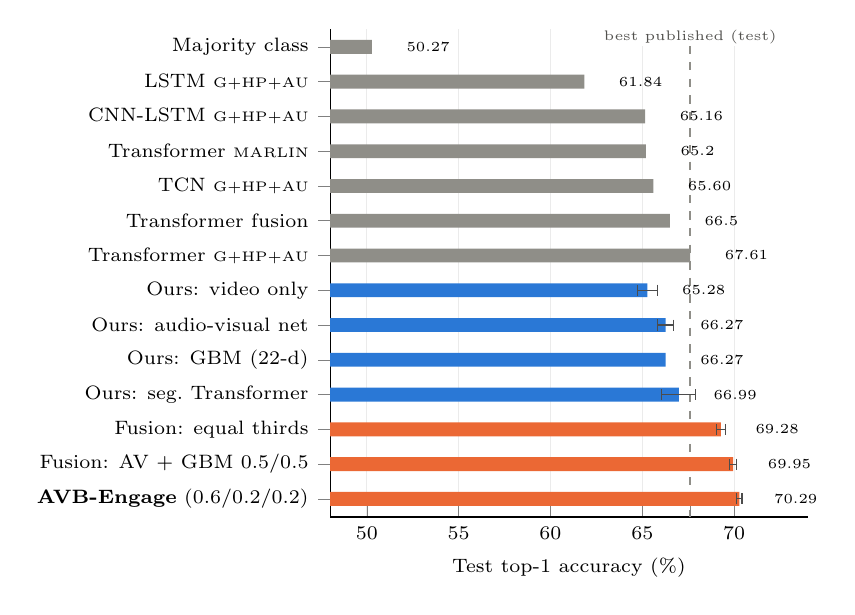
\begin{tikzpicture}
\begin{axis}[
  xbar, bar shift=0pt, scale only axis, width=0.5\columnwidth, height=6.2cm, bar width=5pt,
  xmin=48, xmax=74, xlabel={Test top-1 accuracy (\%)}, xlabel style={font=\scriptsize},
  ytick={maj,lstm,cnnlstm,marlin,tcn,tffus,tfbest,vonly,av,gbm,tf,eq3,av2,w3}, yticklabel style={font=\scriptsize, align=right}, xticklabel style={font=\scriptsize},
  symbolic y coords={maj,lstm,cnnlstm,marlin,tcn,tffus,tfbest,vonly,av,gbm,tf,eq3,av2,w3},
  yticklabels={Majority class,LSTM {\tiny G+HP+AU},CNN-LSTM {\tiny G+HP+AU},Transformer {\tiny MARLIN},TCN {\tiny G+HP+AU},Transformer fusion,Transformer {\tiny G+HP+AU},Ours: video only,Ours: audio-visual net,Ours: GBM (22-d),Ours: seg.\ Transformer,Fusion: equal thirds,Fusion: AV + GBM 0.5/0.5,\textbf{AVB-Engage} (0.6/0.2/0.2)},
  y dir=reverse, enlarge y limits=0.04,
  axis x line*=bottom, axis y line*=left, xmajorgrids, grid style={draw=black!8},
  nodes near coords, nodes near coords style={font=\tiny, text=black, anchor=west, xshift=9pt},
  point meta=explicit symbolic,
  error bars/x dir=both, error bars/x explicit, error bars/error bar style={black!70},
  extra x ticks={67.61}, extra x tick labels={}, extra x tick style={grid=major, grid style={dashed, published, thick}},
]
\addplot[fill=published, draw=none] coordinates {
  (50.27,maj)[50.27] (61.84,lstm)[61.84] (65.16,cnnlstm)[65.16] (65.20,marlin)[65.2]
  (65.60,tcn)[65.60] (66.50,tffus)[66.5] (67.61,tfbest)[67.61]};
\addplot[fill=ours, draw=none] coordinates {
  (65.28,vonly) +- (0.53,0) [65.28] (66.27,av) +- (0.45,0) [66.27]
  (66.27,gbm)[66.27] (66.99,tf) +- (0.93,0) [66.99]};
\addplot[fill=fused, draw=none] coordinates {
  (69.28,eq3) +- (0.23,0) [69.28] (69.95,av2) +- (0.20,0) [69.95] (70.29,w3) +- (0.14,0) [70.29]};
\node[font=\tiny, text=inkmuted, anchor=south, fill=white, inner sep=1pt] at (axis cs:67.61,maj) {best published (test)};
\end{axis}
\end{tikzpicture}

\caption{Test top-1 accuracy on EngageNet. Grey: published video-only baselines \cite{singh2023engagenet}; the dashed line marks the best of them (67.61\%). Blue: our single models. Orange: our probability-level fusions. Error bars are standard deviations over three seeds; the gradient-boosting member is a single averaged model.}
\label{fig_results}
\end{figure}

Table~\ref{tab_baselines} and Fig.~\ref{fig_results} place the proposed models against the six baselines released with EngageNet, all of which operate on video only. These are the only published EngageNet results on the official test split that we are aware of; later work reports validation accuracy (68.91--73.58\%, Section~\ref{sec:relwork}), which is not comparable to test accuracy on this corpus, where validation accuracy runs 1.5--5.2 points above test accuracy for the same baseline model \cite{singh2023engagenet}. Our own validation figures are used for checkpoint, threshold and configuration selection and are therefore optimistic; we report test accuracy throughout. The audio-visual network alone reaches 66.27 $\pm$ 0.45\%, above the LSTM, CNN-LSTM, TCN and MARLIN-Transformer baselines and 1.34 points below the best published figure, which uses hand-engineered gaze, head-pose and action-unit features with a Transformer. Two shallow models on segment statistics of our 22 OpenFace features are as accurate as the whole network on their own (66.27 and 66.99\%). Fusing the three at the probability level with fixed weights gives 70.29 $\pm$ 0.14\%, 2.68 points above the best published test-split result, and 69.28 $\pm$ 0.23\% with equal weights. The gain comes from complementary errors: on seed 1 the network is wrong on 35.9\% of test clips and the gradient-boosting model on 33.5\%, but both are wrong on only 23.5\%.

\begin{table}[!t]
\renewcommand{\arraystretch}{1.3}
\caption{Effect of the Decoding Rule on Identical Trained Weights (Test Top-1, \%, Mean $\pm$ SD Over Three Seeds)}
\label{tab_decoder}
\centering
\resizebox{\columnwidth}{!}{%
\begin{tabular}{|l|c|c|}
\hline
Decoder & Audio + video & Video only\\
\hline
Argmax & 64.27 $\pm$ 0.22 & 63.48 $\pm$ 0.35\\
Fitted logit bias & 65.06 $\pm$ 0.37 & 63.83 $\pm$ 0.45\\
Expected-level thresholds & \textbf{66.34 $\pm$ 0.50} & 65.26 $\pm$ 0.40\\
Refined expected-level thresholds & 66.27 $\pm$ 0.45 & \textbf{65.28 $\pm$ 0.53}\\
\hline
Gain of refined thresholds over argmax & +2.00 & +1.80\\
\hline
\end{tabular}}
\end{table}

Table~\ref{tab_decoder} isolates the decoding rule of Section~\ref{sec:prelim_ordinal}. Replacing argmax with calibrated expected-level thresholds gains 2.00 points of top-1 accuracy for the audio-visual network and 1.80 for its video-only condition, with no change to the weights and no test data used in the fit. This gain is larger than that of any single training change tested in this work (subsection F). Since the decoding rule alone moves reported accuracy by about two points, engagement accuracies from different papers are not comparable unless the decoder is stated; we therefore state it with every figure.

\begin{table}[!t]
\renewcommand{\arraystretch}{1.3}
\caption{Ordinal Metrics on the EngageNet Test Split (Expected-Level Decoding, Mean Over Three Seeds Where Applicable)}
\label{tab_ordinal}
\centering
\resizebox{\columnwidth}{!}{%
\begin{tabular}{|l|c|c|c|c|}
\hline
Model & Top-1 (\%) & Adj.\ (\%) & MAE & Macro-F1\\
\hline
Majority-class predictor & 50.27 & 68.84 & 1.012 & 16.73\\
Network, video only & 65.28 & 90.77 & 0.459 & 51.29\\
Audio-visual network & 66.27 & \textbf{91.55} & 0.440 & 52.31\\
Gradient boosting & 66.27 & 89.01 & 0.480 & 50.04\\
Segment Transformer & 66.99 & 87.90 & 0.487 & 49.45\\
Fusion $(0.6, 0.2, 0.2)$ & \textbf{70.29} & 91.06 & \textbf{0.401} & \textbf{53.95}\\
\hline
\end{tabular}}
\end{table}

Table~\ref{tab_ordinal} reports the full set of ordinal metrics. The audio-visual network has the best adjacent accuracy (91.55\%), and the fusion has the lowest mean absolute class error (0.401) and the highest macro-F1. The size of the adjacent-accuracy figures relative to top-1 shows that the great majority of errors are single-level confusions, a point developed in subsection G.

\subsection{Ablation Analysis}
\label{sec:ablation}

Before reading any ablation, the noise floor must be stated: three independent seeds of one configuration give a standard deviation of 0.45 points of top-1 accuracy and about 1.1 points of macro-F1, and the binomial 95\% confidence interval on 2,256 test clips is roughly $\pm 1.95$ points. We treat a difference in three-seed means below about one point as within noise, and rely on consistency of sign across matched models for smaller effects.

\subsubsection{Modality Contribution on Identical Weights}
Rather than training separate unimodal models, which confounds the contribution of a modality with a different optimisation run, we zero the token sequence of one modality at inference on the already-trained weights (the same operation used as modality dropout during training). Table~\ref{tab_modality} reports the nine fine-tuned networks of this work (three seeds each of the audio-visual network and of the two behavior-branch variants below). Audio alone scores at or below the majority-class predictor on every run, confirming that audio carries no standalone clip-level engagement signal on this corpus. Removing audio from the fused model lowers top-1 accuracy in eight of nine runs, by 0.74 points on average; no single difference clears the noise floor, but the consistency of sign does, and it reproduces an earlier independent sweep in which fusion exceeded the video-only condition in twelve of thirteen matched checkpoints (mean +0.67). Macro-F1 is not consistently improved (five of nine runs). The audio branch therefore contributes through cross-modal interaction rather than through an independent prediction.

\begin{table}[!t]
\renewcommand{\arraystretch}{1.3}
\caption{Inference-Time Modality Ablation on Identical Trained Weights (Nine Networks, Test Top-1, \%)}
\label{tab_modality}
\centering
\resizebox{\columnwidth}{!}{%
\begin{tabular}{|l|c|c|}
\hline
Condition & Mean top-1 & Runs where fusion is better\\
\hline
Audio + video & \textbf{66.16} & --\\
Video only & 65.41 & 8 of 9 ($+0.74$)\\
Audio only & 48.60 & 9 of 9 (at or below majority)\\
\hline
\end{tabular}}
\end{table}

% TODO (alignment ablation): the earlier with/without-alignment table was measured on a test set that had been
% extracted at 15 frames per clip (defect fixed 2026-08-07) and has been removed. Re-run the matched
% no-alignment arm on the corrected 50-frame data (3 seeds) before making any claim about the effect of alignment.

\subsubsection{Neural Behavior Branch}
The neural behavior branch of Section~\ref{sec:method}-B was attached to the same warm start as the audio-visual network, with the same frame cap, schedule and seeds, and with its new classifier columns initialised to zero. Over three seeds it scores 66.08 $\pm$ 0.59\% top-1, 91.62\% adjacent accuracy, 0.441 MAE and 52.16 macro-F1, against 66.27 $\pm$ 0.45\%, 91.55\%, 0.440 and 52.31 for the audio-visual network: no metric moves by more than a fraction of the seed standard deviation, under any of the four decoders. Adding a textual rendering of the same action-unit series as a further input stream also leaves every metric unchanged (66.12 $\pm$ 0.59\%). A per-subject baseline subtraction of the descriptors was also tested and lowered top-1 accuracy by 1.05 points. The behavior features are nonetheless informative: the segment-statistics members of Section~\ref{sec:latefusion} reach 66.3--67.0\% on the same 22 features, and replacing the audio-visual network by the behavior-branch network as the neural member of the three-way fusion gives the same 69.9--70.4\% range. The limitation is therefore the per-frame recurrent encoding of the branch, not the features.

\subsubsection{Late-Fusion Members and Weight Selection}
Table~\ref{tab_fusion} reports the fusion of the audio-visual network with the behavior-statistics members under several weight rules. Fixed weights require no selection and are the numbers we report; validation-selected weights are shown as a check. Every rule and every seed lands between 67.4\% and 70.5\%; the two low values occur when validation selected an extreme weight on the network (0.85 or 0.8) for one seed. A two-way fusion of the network with the segment Transformer alone is unstable (68.69 $\pm$ 2.08\% with validation-selected weights) because the Transformer's validation accuracy tracks its test accuracy poorly; the gradient-boosting member stabilises the fusion. Replacing the 22-dimensional descriptor by the full 98-dimensional descriptor of the published baseline raises the gradient-boosting member alone to 68.88\% (68.13\% with argmax decoding), above the published Transformer on the same features, but does not improve the fusion (69.15 $\pm$ 0.83\% three-way with validation-selected weights).

\begin{table}[!t]
\renewcommand{\arraystretch}{1.25}
\caption{Late Fusion With the Audio-Visual Network Under Different Weight Rules (Test Top-1, \%, Three Seeds)}
\label{tab_fusion}
\centering
\resizebox{\columnwidth}{!}{%
\begin{tabular}{|l|l|c|}
\hline
Members & Weight rule & Top-1\\
\hline
AV + GBM & fixed 0.5 / 0.5 & 69.95 $\pm$ 0.20\\
AV + GBM & fixed 0.7 / 0.3 & 70.04 $\pm$ 0.20\\
AV + GBM & selected on validation & 69.86 $\pm$ 0.50\\
AV + TF + GBM & fixed equal thirds & 69.28 $\pm$ 0.23\\
AV + TF + GBM & fixed 0.6 / 0.2 / 0.2 & \textbf{70.29 $\pm$ 0.14}\\
AV + TF + GBM & selected on validation & 69.43--70.29\\
\hline
\end{tabular}}
\end{table}

\subsubsection{Training Variables and the Noise Floor}
Fourteen fine-tuning runs of the audio-visual network were warm-started from the same checkpoint, each changing exactly one training variable: loss type (ordinal versus plain cross-entropy), ordinal penalty weight (0.15, 0.35, 0.60), class-weighted loss, class-balanced sampling, learning-rate schedule, exponential moving average of weights, label smoothing, SpecAugment on the spectrogram, the video frame cap, and synchronised random temporal cropping. Table~\ref{tab_sweep} lists the results. Every isolated comparison is null: the spread across all fourteen configurations (standard deviation 0.52) is no larger than the spread across three seeds of one configuration (0.45). Augmentation is the only variable with a clear direction, and it is harmful (64.89 against its otherwise-identical pair at 65.82). Averaging the logits of all fourteen checkpoints scores 65.69, below the best single model, because members sharing a warm start make correlated errors. We read these three observations together as evidence that, for a single end-to-end network on this corpus, training variables are exhausted; the gains reported above come instead from a better decoder and from combining different representations.

\begin{table}[!t]
\renewcommand{\arraystretch}{1.2}
\caption{Single-Variable Fine-Tuning Sweep From a Shared Warm Start (Test Split, Refined Decoder)}
\label{tab_sweep}
\centering
\resizebox{\columnwidth}{!}{%
\begin{tabular}{|l|c|c|c|c|}
\hline
Variable under test & Top-1 & Adjacent & MAE & Macro-F1\\
\hline
Control & 66.09 & 91.40 & 0.444 & 52.25\\
Balanced sampler, seed 1 & 65.78 & \textbf{92.24} & \textbf{0.436} & \textbf{53.41}\\
Balanced sampler, seed 2 & 66.36 & 91.09 & 0.444 & 51.13\\
Balanced sampler, seed 3 & \textbf{66.67} & 91.31 & 0.440 & 52.37\\
Loss = cross-entropy & 65.91 & 91.36 & 0.446 & 50.92\\
Ordinal weight 0.35 & 65.38 & 91.27 & 0.452 & 50.68\\
Ordinal weight 0.60 & 65.87 & 91.36 & 0.446 & 50.94\\
No label smoothing & 65.91 & 91.44 & 0.445 & 51.01\\
EMA 0.999 & 65.96 & 91.22 & 0.446 & 50.93\\
LR $10^{-4}$, warm-up cosine & 65.69 & 91.36 & 0.448 & 50.72\\
SpecAugment & 65.34 & 91.22 & 0.453 & 50.59\\
Frame cap 50 & 65.82 & 91.40 & 0.446 & 50.76\\
Frame cap 40 + synced random crop & 64.89 & 91.53 & 0.450 & 50.42\\
Class-weighted loss & 64.72 & 91.71 & 0.452 & 50.41\\
\hline
Ensemble of all 14 & 65.69 & -- & -- & --\\
\hline
\end{tabular}}
\end{table}

\subsection{Error Analysis on the Hard Categories}

Fig.~\ref{fig_confusion} shows the row-normalised test confusion matrices of the audio-visual network and of the three-way fusion, pooled over the three seeds. The two extreme levels are recognised well by the network (79\% and 85\%), whereas the two middle levels, \emph{barely engaged} and \emph{engaged}, are recognised at only 12\% and 30\%. Three quarters of the network's errors are off by exactly one level, and 65.8\% of them fall on clips whose true level is one of the two middle levels, which together make up only 29.5\% of the test set. Fusion does not change this picture: it raises recall on \emph{highly engaged} (85\% to 94\%) and \emph{engaged} (30\% to 38\%) at the cost of \emph{not engaged} (79\% to 73\%), \emph{barely engaged} stays near 11\%, and 71.8\% of its remaining errors are on the middle levels.

\begin{figure}[!t]
\centering
% Fig. — row-normalised test confusion matrices, pooled over the three seeds of arm A (3 x 2,256 clips).
% Generated from results/fullclip (A_av_s*/context/logits.npz and segtf/fusion_A_av_s*_3way.json).
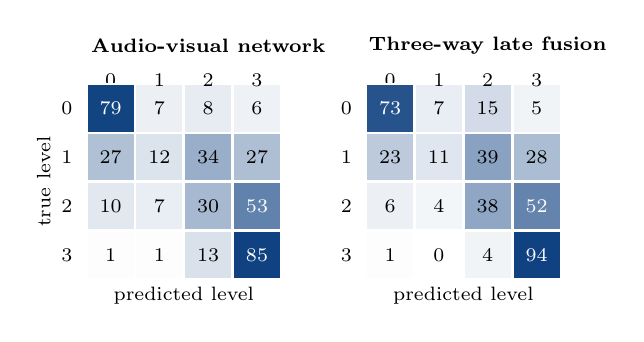
\begin{tikzpicture}[font=\scriptsize, cell/.style={minimum size=0.62cm, inner sep=0pt, draw=white, line width=1pt}]
\node[font=\scriptsize\bfseries] at (1.24,0.8) {Audio-visual network};
\node[anchor=east] at (-0.36,0.00) {0};
\node at (0.00,0.36) {0};
\node[cell, fill=seqhi!99!seqlo, text=white] at (0.00,0.00) {79};
\node[cell, fill=seqhi!8!seqlo, text=black] at (0.62,0.00) {7};
\node[cell, fill=seqhi!10!seqlo, text=black] at (1.24,0.00) {8};
\node[cell, fill=seqhi!7!seqlo, text=black] at (1.86,0.00) {6};
\node[anchor=east] at (-0.36,-0.62) {1};
\node at (0.62,0.36) {1};
\node[cell, fill=seqhi!33!seqlo, text=black] at (0.00,-0.62) {27};
\node[cell, fill=seqhi!15!seqlo, text=black] at (0.62,-0.62) {12};
\node[cell, fill=seqhi!43!seqlo, text=black] at (1.24,-0.62) {34};
\node[cell, fill=seqhi!34!seqlo, text=black] at (1.86,-0.62) {27};
\node[anchor=east] at (-0.36,-1.24) {2};
\node at (1.24,0.36) {2};
\node[cell, fill=seqhi!12!seqlo, text=black] at (0.00,-1.24) {10};
\node[cell, fill=seqhi!9!seqlo, text=black] at (0.62,-1.24) {7};
\node[cell, fill=seqhi!37!seqlo, text=black] at (1.24,-1.24) {30};
\node[cell, fill=seqhi!66!seqlo, text=white] at (1.86,-1.24) {53};
\node[anchor=east] at (-0.36,-1.86) {3};
\node at (1.86,0.36) {3};
\node[cell, fill=seqhi!1!seqlo, text=black] at (0.00,-1.86) {1};
\node[cell, fill=seqhi!1!seqlo, text=black] at (0.62,-1.86) {1};
\node[cell, fill=seqhi!16!seqlo, text=black] at (1.24,-1.86) {13};
\node[cell, fill=seqhi!100!seqlo, text=white] at (1.86,-1.86) {85};
\node at (0.93,-2.38) {predicted level};
\node[font=\scriptsize\bfseries] at (4.79,0.8) {Three-way late fusion};
\node[anchor=east] at (3.19,0.00) {0};
\node at (3.55,0.36) {0};
\node[cell, fill=seqhi!91!seqlo, text=white] at (3.55,0.00) {73};
\node[cell, fill=seqhi!9!seqlo, text=black] at (4.17,0.00) {7};
\node[cell, fill=seqhi!19!seqlo, text=black] at (4.79,0.00) {15};
\node[cell, fill=seqhi!6!seqlo, text=black] at (5.41,0.00) {5};
\node[anchor=east] at (3.19,-0.62) {1};
\node at (4.17,0.36) {1};
\node[cell, fill=seqhi!28!seqlo, text=black] at (3.55,-0.62) {23};
\node[cell, fill=seqhi!13!seqlo, text=black] at (4.17,-0.62) {11};
\node[cell, fill=seqhi!49!seqlo, text=black] at (4.79,-0.62) {39};
\node[cell, fill=seqhi!35!seqlo, text=black] at (5.41,-0.62) {28};
\node[anchor=east] at (3.19,-1.24) {2};
\node at (4.79,0.36) {2};
\node[cell, fill=seqhi!8!seqlo, text=black] at (3.55,-1.24) {6};
\node[cell, fill=seqhi!5!seqlo, text=black] at (4.17,-1.24) {4};
\node[cell, fill=seqhi!47!seqlo, text=black] at (4.79,-1.24) {38};
\node[cell, fill=seqhi!65!seqlo, text=white] at (5.41,-1.24) {52};
\node[anchor=east] at (3.19,-1.86) {3};
\node at (5.41,0.36) {3};
\node[cell, fill=seqhi!1!seqlo, text=black] at (3.55,-1.86) {1};
\node[cell, fill=seqhi!0!seqlo, text=black] at (4.17,-1.86) {0};
\node[cell, fill=seqhi!6!seqlo, text=black] at (4.79,-1.86) {4};
\node[cell, fill=seqhi!100!seqlo, text=white] at (5.41,-1.86) {94};
\node at (4.48,-2.38) {predicted level};
\node[rotate=90] at (-0.85,-0.93) {true level};
\end{tikzpicture}

\caption{Row-normalised test confusion matrices (\%) for the audio-visual network (left) and the three-way late fusion (right), pooled over three seeds ($3 \times 2{,}256$ clips). Levels: 0 not engaged, 1 barely engaged, 2 engaged, 3 highly engaged. Most errors are one-level confusions involving the two middle levels.}
\label{fig_confusion}
\end{figure}

\begin{table}[!t]
\renewcommand{\arraystretch}{1.3}
\caption{Effect of Label Granularity (One Audio-Visual Network, Argmax Decoder, No Retraining)}
\label{tab_perclass}
\centering
\resizebox{\columnwidth}{!}{%
\begin{tabular}{|l|c|c|c|}
\hline
Label granularity & Top-1 (\%) & Majority (\%) & Gain\\
\hline
4 levels (as trained) & 64.27 & 50.3 & +13.97\\
3 levels (middle two merged) & 70.70 & 50.3 & \textbf{+20.40}\\
2 levels (disengaged vs.\ engaged) & 85.95 & 68.9 & +17.05\\
\hline
\end{tabular}}
\end{table}

We think there are two reasons for this behavior. First, the two middle levels describe a difference of degree in the same visible behavior: a student who is looking at the screen with a neutral face may be barely engaged or engaged, and a ten-second window gives no additional evidence, such as speech or a response to the instructor, that would separate them. Second, the annotation itself is least reliable at this boundary, since human raters also disagree most between adjacent middle levels. Table~\ref{tab_perclass} supports this reading: merging the two middle levels of the same trained network, with no retraining, raises the gain over the corresponding majority baseline from 13.97 to 20.40 points, a larger improvement than any single training change in this work. A second, smaller source of error is a shift in the label prior between the splits: the validation split contains 12.3\% \emph{not engaged} clips against 20.3\% in the test split, and thresholds fitted on the test split itself would score 67.82\% instead of 65.69\% for one network (an oracle bound, not a method). The practical conclusion is that the remaining difficulty on EngageNet lies in the middle of the scale, and that speech-rich data with a role-aware label scheme, where listening and speaking are annotated separately, is the most promising way to resolve it.

\subsection{Qualitative Study: Human Evaluation}

A human evaluation is a necessary complement to the numerical metrics above, because the ground truth of engagement is itself a human judgement and the metrics cannot tell whether the model's hard categories are also hard for people. The study follows the design of the annotation itself. A stratified sample of 200 test clips, 50 per level, is shown to a panel of raters with teaching experience, who assign an engagement level using the same four anchors given to the EngageNet annotators and additionally mark whether the student appears to be speaking or listening. Three quantities are then computed: inter-rater agreement (Krippendorff's $\alpha$ with ordinal weighting), rater-versus-label agreement on the same scale, and the confusion matrix of the raters against the labels, which is compared level by level with the confusion matrix of the model (Fig.~\ref{fig_confusion}). If the raters confuse the two middle levels at a rate similar to the model, the residual error in subsection G is a property of the label space rather than of the architecture; if they separate the middle levels better than the model, the gap identifies information that is visible to humans and not yet used by the model, which the speaking-or-listening mark is designed to expose. This study has not yet been run; the protocol is fixed here so that its outcome is pre-registered. It will be conducted first on the EngageNet sample and then on recordings of a live online course with breakout-room discussion, where per-participant audio is available and the speaking condition can be verified.
% TODO: add the survey results table once the panel study is complete (plan.md §18.5).

% \section{Conclusion and Future Scope}
% Write after the results tables are final: best model, key ablations,
% limitations, and future work without repeating the abstract.

% \section*{Acknowledgment}

\ifCLASSOPTIONcaptionsoff
  \newpage
\fi

\begin{thebibliography}{99}

\bibitem{singh2023engagenet}
M.~Singh, X.~Hoque, D.~Zeng, Y.~Wang, K.~Ikeda, and A.~Dhall, ``Do I have your attention: A large scale engagement prediction dataset and baselines,'' in \emph{Proc. 25th Int. Conf. Multimodal Interaction (ICMI)}, Paris, France, 2023, pp.~174--182, doi: 10.1145/3577190.3614164.

\bibitem{wu2024cmose}
C.-H.~Wu, S.-Y.~Liu, X.~Huang, X.~Wang, R.~Zhang, L.~Minciullo, W.~K.~Yiu, K.~Kwan, and K.-T.~Cheng, ``CMOSE: Comprehensive multi-modality online student engagement dataset with high-quality labels,'' in \emph{Proc. IEEE/CVF Conf. Comput. Vis. Pattern Recognit. Workshops (CVPRW)}, 2024, pp.~4636--4645, doi: 10.1109/CVPRW63382.2024.00466.

\bibitem{tran2026ordinal}
N.~Tran, D.~Ly, P.~Ta, H.~Nguyen, and H.~D.~Nguyen, ``Ordinal-aware multimodal engagement recognition for collaborative learning,'' in \emph{Proc. IEEE/CVF Winter Conf. Appl. Comput. Vis. (WACV)}, 2026, pp.~2424--2433, doi: 10.1109/WACV61042.2026.00239.

\bibitem{qarbal2025review}
I.~Qarbal, N.~Sael, and S.~Ouahabi, ``Student's engagement detection based on computer vision: A systematic literature review,'' \emph{IEEE Access}, vol.~13, pp.~140519--140545, 2025, doi: 10.1109/ACCESS.2025.3596885.

\bibitem{gupta2016daisee}
A.~Gupta, A.~D'Cunha, K.~Awasthi, and V.~Balasubramanian, ``DAiSEE: Towards user engagement recognition in the wild,'' arXiv:1609.01885, 2016.

\bibitem{venkatraman2025avtca}
J.~Dhanith~P.~R., S.~Venkatraman, V.~Sharma, and S.~Malarvannan, ``Multimodal emotion recognition using audio-video transformer fusion with cross attention,'' arXiv:2407.18552v4, Jan. 2026.

\bibitem{nagrani2021attention}
A.~Nagrani, S.~Yang, A.~Arnab, A.~Jansen, C.~Schmid, and C.~Sun, ``Attention bottlenecks for multimodal fusion,'' in \emph{Advances in Neural Information Processing Systems}, vol.~34, 2021.

\bibitem{mo2024earlyfusion}
S.~Mo and P.~Morgado, ``Unveiling the power of audio-visual early fusion transformers with dense interactions through masked modeling,'' in \emph{Proc. IEEE/CVF Conf. Comput. Vis. Pattern Recognit. (CVPR)}, 2024, pp.~27176--27186, doi: 10.1109/CVPR52733.2024.02567.

\bibitem{qin2026glpfusion}
Z.~Qin, S.~Shen, D.~Sun, K.~Zhu, Z.~Huang, Q.~Liu, and S.~Wang, ``GLP-fusion: A hierarchical multimodal fusion framework for robust student engagement prediction,'' \emph{IEEE Trans. Multimedia}, early access, 2026, doi: 10.1109/TMM.2026.3685539.

\bibitem{zhao2021efficientface}
Z.~Zhao, Q.~Liu, and F.~Zhou, ``Robust lightweight facial expression recognition network with label distribution training,'' in \emph{Proc. AAAI Conf. Artif. Intell.}, vol.~35, no.~4, 2021, pp.~3510--3519.

\bibitem{baltrusaitis2018openface}
T. Baltru\v{s}aitis, A. Zadeh, Y. C. Lim, and L.-P. Morency, ``OpenFace 2.0: Facial behavior analysis toolkit,'' in \emph{Proc. IEEE Int. Conf. Autom. Face Gesture Recognit. (FG)}, 2018, pp. 59--66.

\bibitem{livingstone2018ravdess}
S.~R.~Livingstone and F.~A.~Russo, ``The Ryerson audio-visual database of emotional speech and song (RAVDESS): A dynamic, multimodal set of facial and vocal expressions in North American English,'' \emph{PLoS ONE}, vol.~13, no.~5, Art.~no.~e0196391, 2018.

\bibitem{theophilus2026review}
G.~Theophilus, C.~I.~Eke, O.~J.~Agushaka, and T.~Moses, ``Shallow and deep learning approaches for predicting learners' engagement in electronic learning systems: Feature selection, extraction and engineering approaches,'' \emph{Neural Comput. Appl.}, vol.~38, no.~9, Art.~no.~323, 2026, doi: 10.1007/s00521-026-11987-3.

\bibitem{yulius2025gan}
R. Yulius, S. Sumpeno, and M. H. Purnomo, ``Making the silent seen: GAN augmentation for low-engagement detection,'' in \emph{Proc. Int. Conf. Computer Engineering, Network and Intelligent Multimedia (CENIM)}, 2025, pp. 243--248, doi: 10.1109/CENIM67940.2025.11325760.

\bibitem{xie2025msctrans}
N. Xie, Z. Li, H. Lu, W. Pang, J. Song, and B. Lu, ``MSC-Trans: A multi-feature-fusion network with encoding structure for student engagement detecting,'' \emph{IEEE Transactions on Learning Technologies}, vol. 18, pp. 243--255, 2025, doi: 10.1109/TLT.2025.3530457.

\bibitem{zhao2026multimodal}
D.~Zhao, Y.~Zhao, and T.~Zhao, ``A multimodal AI framework for real-time student engagement detection and adaptive feedback in higher education,'' \emph{J. King Saud Univ. -- Comput. Inf. Sci.}, vol.~38, no.~5, Art.~no.~243, 2026, doi: 10.1007/s44443-026-00639-0.

\bibitem{li2026mersurvey}
H.~Li, H.~Han, C.~Xu, T.~Chen, X.~Liu, and G.~Wen, ``Multimodal emotion recognition from complete modality to missing modality based on text, audio, and visual: A review,'' \emph{Eng. Appl. Artif. Intell.}, vol.~170, Art.~no.~114127, 2026, doi: 10.1016/j.engappai.2026.114127.

\bibitem{taware2025mer}
S.~Taware and A.~D.~Thakare, ``Multimodal emotion recognition based on face and speech using deep convolution neural network and long short term memory,'' \emph{Circuits Syst. Signal Process.}, vol.~44, no.~9, pp.~6622--6649, 2025, doi: 10.1007/s00034-025-03080-2.

\bibitem{hegde2025sentiment}
R. Hegde and S. K. Hegde, ``Multi-modal deep learning for comprehensive polarity detection and sentiment analysis,'' in \emph{Proc. 8th Int. Conf. Computing Methodologies and Communication (ICCMC)}, 2025, pp. 663--668, doi: 10.1109/ICCMC65190.2025.11140986.

\bibitem{lu2026dstc}
J. Lu, Y. Shang, Z. Shao, T. Liu, H. Ding, and Q. Hu, ``DSTC: A multimodal network for depression emotion recognition and sentiment analysis,'' \emph{IEEE Transactions on Affective Computing}, vol. 17, no. 1, pp. 630--642, 2026, doi: 10.1109/TAFFC.2025.3628664.

\bibitem{kim2024avaction}
J.-H. Kim and C. S. Won, ``Audio-visual action recognition using transformer fusion network,'' \emph{Applied Sciences}, vol. 14, no. 3, p. 1190, 2024, doi: 10.3390/app14031190.


\bibitem{vedernikov2024tcct}
A.~Vedernikov, P.~Kumar, H.~Chen, T.~Sepp\"{a}nen, and X.~Li, ``TCCT-Net: Two-stream network architecture for fast and efficient engagement estimation via behavioral feature signals,'' in \emph{Proc. IEEE/CVF Conf. Comput. Vis. Pattern Recognit. Workshops (CVPRW)}, 2024, pp.~4723--4732, doi: 10.1109/CVPRW63382.2024.00475.

\bibitem{abedi2024stgcn}
A.~Abedi and S.~S.~Khan, ``Engagement measurement based on facial landmarks and spatial-temporal graph convolutional networks,'' in \emph{Proc. Int. Conf. Pattern Recognit. (ICPR)}, Lecture Notes in Computer Science. Cham, Switzerland: Springer, 2024, pp.~321--338, doi: 10.1007/978-3-031-78201-5\_21.

\bibitem{vedernikov2026priornet}
A.~Vedernikov, ``PriorNet: Prior-guided engagement estimation from face video,'' \emph{Mach. Vis. Appl.}, vol.~37, no.~6, Art.~no.~154, 2026, doi: 10.1007/s00138-026-01918-6.

\bibitem{vedernikov2025vlmnoise}
A.~Vedernikov, P.~Kumar, H.~Chen, T.~Sepp\"{a}nen, and X.~Li, ``Vision large language models are good noise handlers in engagement analysis,'' arXiv:2511.14749, 2025.

\bibitem{augusma2026vemd}
A.~Augusma, D.~Vaufreydaz, and F.~Letu\'{e}, ``Variational encoder--multi-decoder (VE-MD) for privacy-by-functional-design (group) emotion recognition,'' arXiv:2604.02397, 2026.

\bibitem{safa2025sclordinal}
S.~Safa, A.~Abedi, and S.~S.~Khan, ``Supervised contrastive learning for ordinal engagement measurement,'' in \emph{Proc. Conf. Robots and Vision (CRV)}, 2025, doi: 10.21428/d82e957c.e69751f0.

\bibitem{abedi2024affect}
A.~Abedi and S.~S.~Khan, ``Affect-driven ordinal engagement measurement from video,'' \emph{Multimedia Tools Appl.}, vol.~83, no.~8, pp.~24899--24918, 2024, doi: 10.1007/s11042-023-16345-2.

\bibitem{gothwal2025vibednet}
P.~Gothwal, D.~Banerjee, and A.~K.~Biswas, ``ViBED-Net: Video based engagement detection network using face-aware and scene-aware spatiotemporal cues,'' arXiv:2510.18016, 2025.

\bibitem{das2025optimizing}
R.~Das and S.~Dev, ``Optimizing student engagement detection using facial and behavioral features,'' \emph{Neural Comput. Appl.}, vol.~37, no.~23, pp.~19063--19085, 2025, doi: 10.1007/s00521-025-11317-z.

\end{thebibliography}

% \begin{IEEEbiographynophoto}{Author Name}
% Biography text here.
% \end{IEEEbiographynophoto}

\end{document}
